\chapter{Descrierea aplicației}

În acest capitol voi descrie pe scurt aplicația SPA creată
pentru lucrarea de licență.

\section{Scop și prezentare generală}

Aplicația este un \emph{expense tracker},
adică permite unui utilizator să țină evidența
cheltuielilor. Ea permite unui utilizator 
să se înregistreze sau să se logheze,
apoi acesta are acces la operațiile
CRUD (Create Read Update Delete) asupra cheltuielilor sale.

Aplicația permite și căutarea cheieltuierilor
după cuvinte ce se găsesc în descrierea acestora,
sau filtrarea după dată. De asemenea se pot printa
toate cheltuielile dintr-o săptămână.


\section{Instalare aplicație și pornire server de dezvoltare}

Următorii pași trebuie urmați pentru pornirea server-ului
de dezvoltare pe un sistem Linux / Mac OS X:
\begin{enumerate}
\item Se clonează proiectul folosind comanda
"git clone https://github.com/stefan-mihaila/money-keep".
\item Se schimbă directorul curent în cel al aplicației: "cd money-keep".
\item Se recomandă crearea unui mediu izolat pentru 
instalarea pachetelor Python necesare aplicației.
Pentru asta, se foloseștie comanda "pip install virtualenv"
pentru instalarea utilitarului \emph{virtualenv}
și comanda "virtualenv create env" pentru crearea
mediului virtual. Apoi se activează acest mediu
folosind "source env/bin/activate". De acum încolo,
comenzile "python" și "pip" nu mai sunt cele instalate
global în sistem, ci cele din "env/bin/". Pentru dezactivarea
mediului virtual se rulează "deactivate".
\item Se instalează pachetele adiționale Python folosite 
(incluzând Django). Aceste pachete sunt enumerate în fișierul
'requirements.txt'. Toate pachetele din acest fișier pot
fi instalate rulând comanda "pip install -r requirements.txt".
\item Se rulează migrațiile cu comanda "./manage.py migrate".
\item Se instalează Node.js și \texttt{npm}. Instrucțiuni de instalare se găsesc aici:
\url{https://nodejs.org}. \texttt{npm} este necesar pentru a instala \texttt{Bower}.
\item Se instalează \texttt{Bower} folosind comanda "npm install -g bower".
\item Se instalează dependențele de front-end folosind comanda
"bower install". Această comandă instalează dependențele listate
în "bower.json".
\item Se poate porni serverul cu comanda "./manage.py runserver". Dacă
totul a mers bine, serverul acceptă request-uri la adresa \url{http://127.0.0.1:8000}.
\end{enumerate}

Comanda \texttt{./manage.py migrate} de mai sus a creat baza de date
a aplicației. Baza de date este configurată în fișierul 
\texttt{money\_keep/settings.py}:

\begin{lstlisting}[language=python, title=Configurare implicită a bazei de date]
DATABASES = {
    'default': {
        'ENGINE': 'django.db.backends.sqlite3',
        'NAME': os.path.join(BASE_DIR, 'db.sqlite3'),
    }
}
\end{lstlisting}

După cum se observă, în mod implicit se folosește \emph{SQLite}.
SQLite este o bază de date ce își ține toate tabelele într-un
singur fișier (\texttt{db.sqlite3} în cazul nostru). Am ales
să folosesc această bază de date pentru dezvoltare
deoarece este foarte ușor de folosit / administrat.
Pentru a se folosi o bază de date "mai serioasă", este necesar
doar să fie instalată baza de date și să se modifice dicționarul
\texttt{DATABASES} din \texttt{settings.py}.


\section{Folosirea aplicației}

Se face click pe "Register", apoi se completează formularul cu 
email-ul, numele utilizatorului și parola (vezi Figura \ref{fig:register}).
După click pe "Submit", utilizatorul este creat și logat în aplicație.

\begin{figure}
  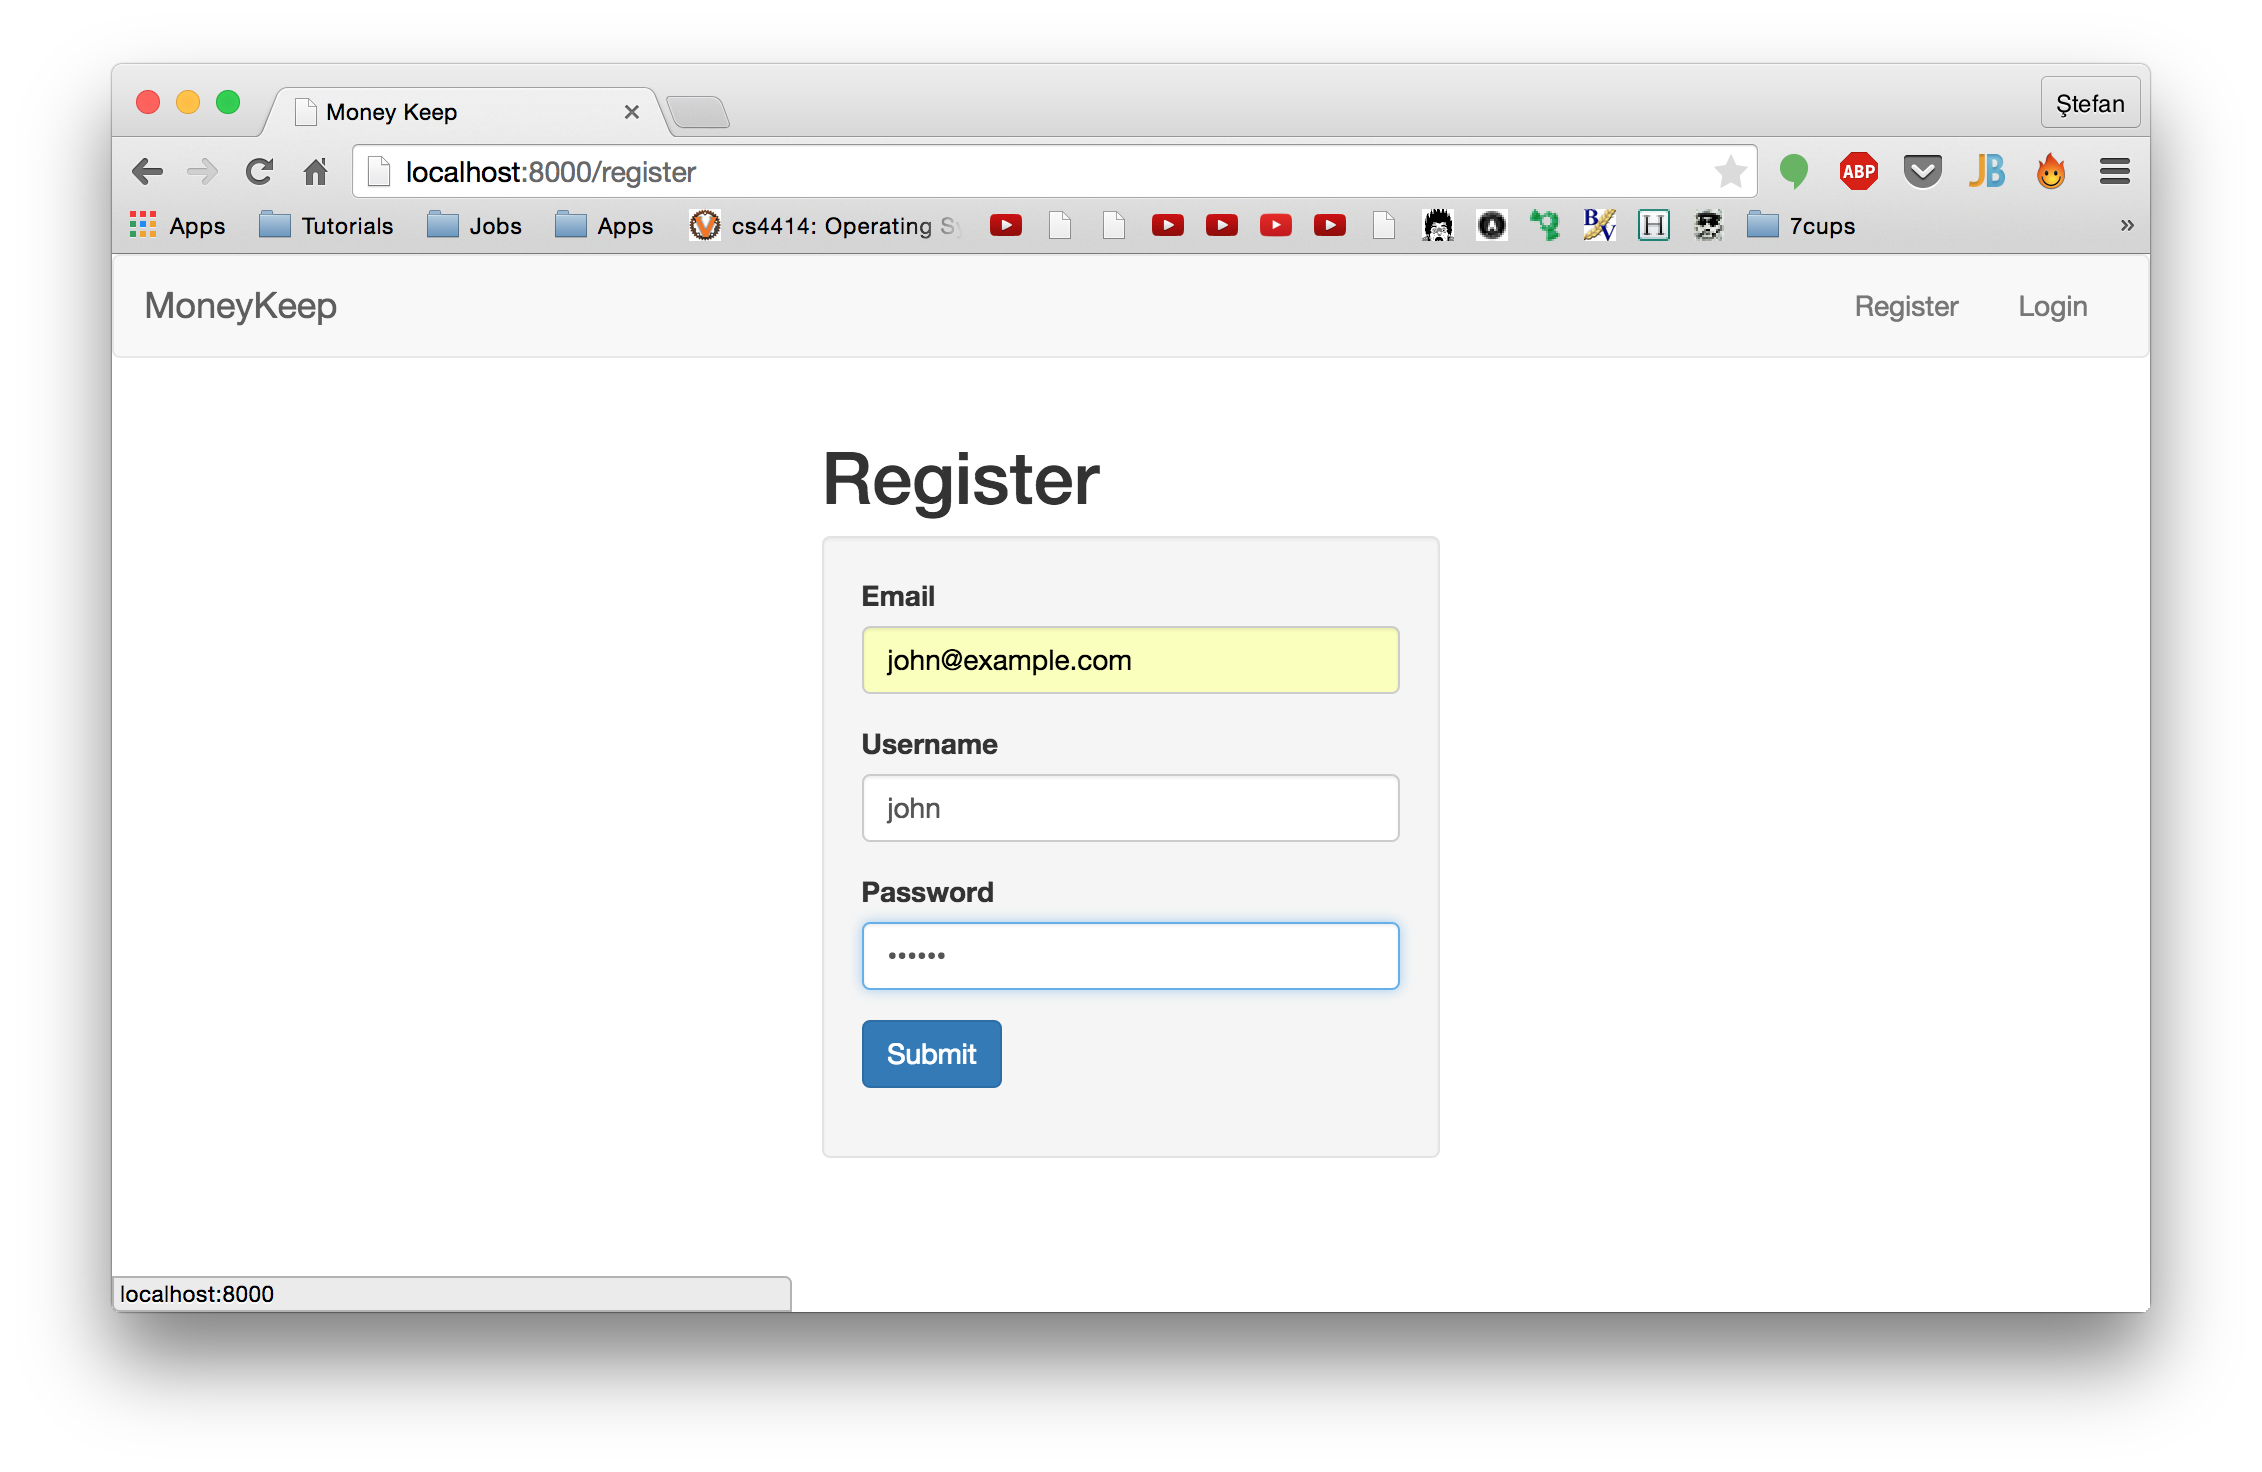
\includegraphics[width=1\textwidth]{./chap5-files/register}
  \caption{Crearea unui utilizator nou}
  \label{fig:register}
\end{figure}

\begin{figure}
  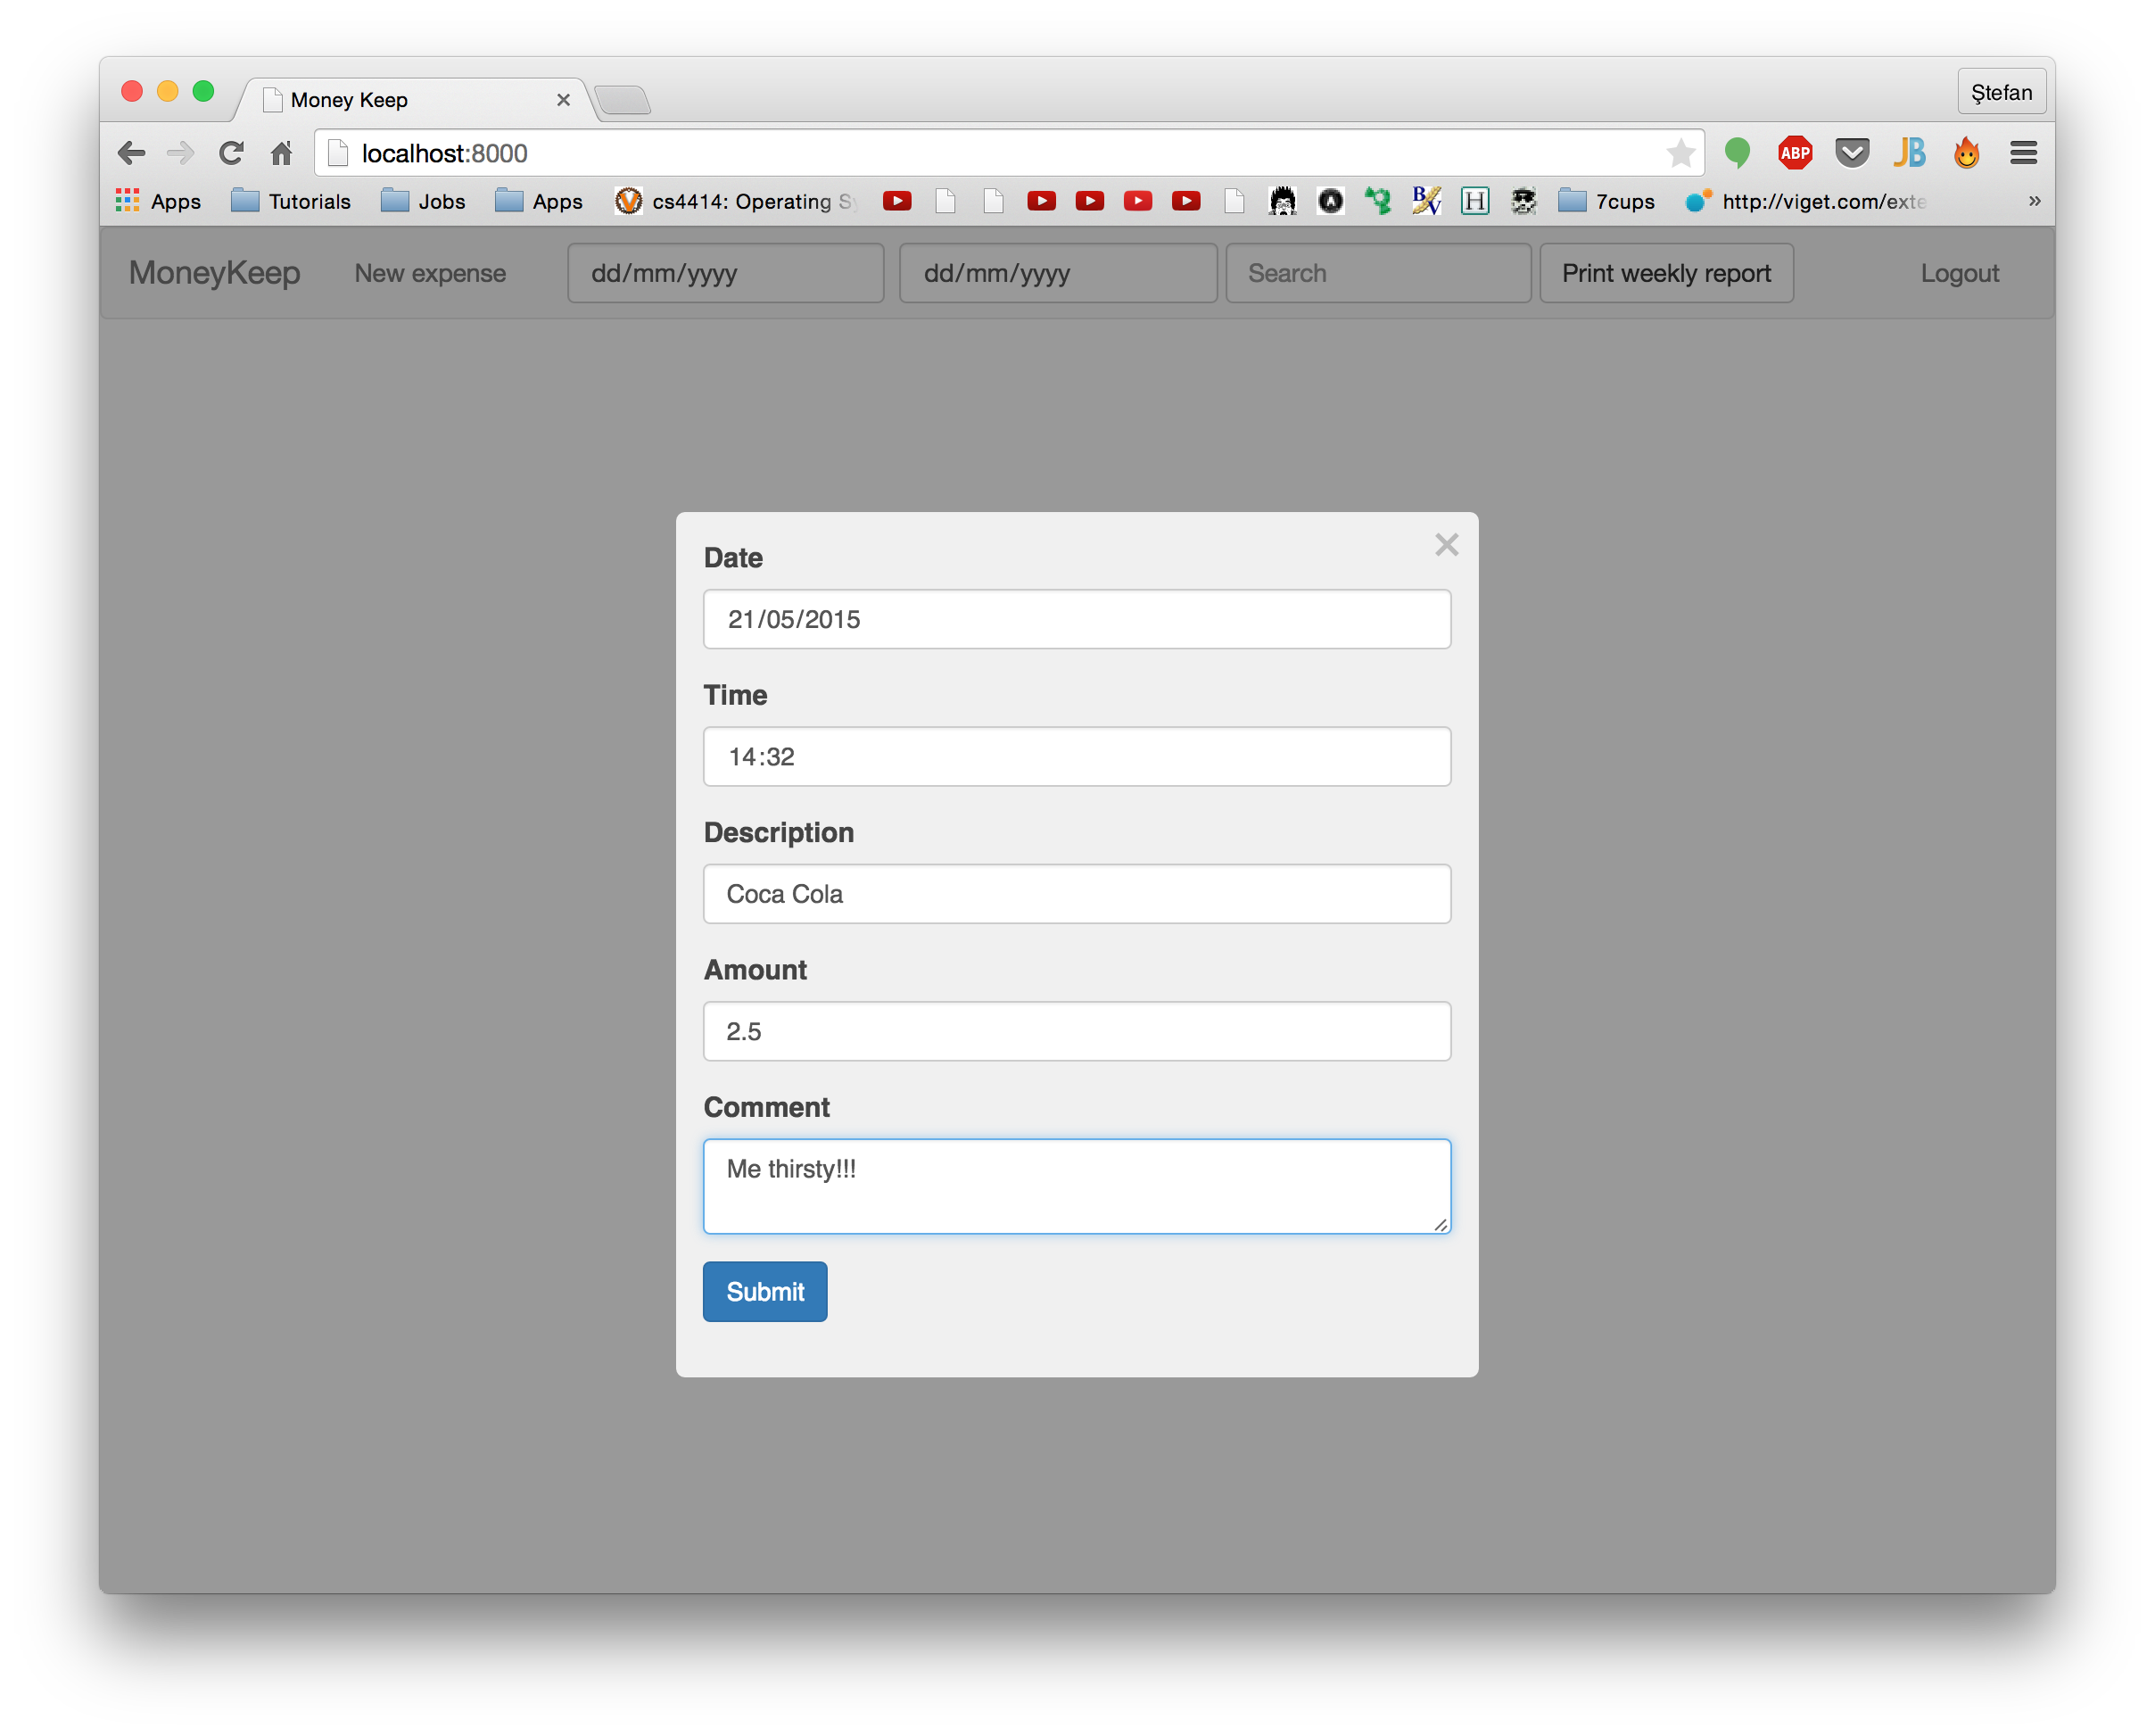
\includegraphics[width=1\textwidth]{./chap5-files/new-expense}
  \caption{Adăugarea unei cheltuieli noi}
  \label{fig:new-expense}
\end{figure}

După ce s-a logat, utilizatorul poate adăuga o nouă cheltuială în aplicație
dând click pe "New expense". Acesta este rugat să introducă detaliile
cheltuielii: data, ora, descrierea, suma și un comentariu opțional
(vezi Figura \ref{fig:new-expense}).

După ce au fost adăugate cheltuieli, acestea pot fi editate sau șterse.
De asemenea, cheltuielile pot fi filtrate după dată sau se pot
efectua căutări după cuvinte ce se găsesc în titlul sau comentariul
cheltuielilor. Există și opțiunea de a printa cheltuielile dintr-o
anumită săptămână.


